\documentclass[logo,reportComp]{thesis}
\usepackage[python,pseudo,linenum]{mypackage}
\usepackage{pythonhighlight}

\title{机器学习与数据挖掘大作业}
\subtitle{多标签用户人格分类(SVM)}
\school{数据科学与计算机学院}
\author{陈鸿峥}
\classname{17大数据与人工智能}
\stunum{17341015}
\headercontext{机器学习与数据挖掘大作业}

\let\emph\relax % there's no \RedeclareTextFontCommand
\DeclareTextFontCommand{\emph}{\kaiti\em}

\begin{document}

\maketitle
\tableofcontents

\newpage
\section{题目描述}
MBTI理论认为一个人的个性可以从四个角度进行分析,用字母代表如下:
\begin{itemize}
    \item 驱动力的来源:外向E---内向I
    \item 接受信息的方式:感觉S---直觉N
    \item 决策的方式:思维T---情感F
    \item 对待不确定性的态度:判断J---知觉P
\end{itemize}
按照不同的组合,可以产生16种人格类型。

本次大作业要求利用机器学习方法,通过用户的发言记录对用户的人格类型进行分类\footnote{数据集链接:\url{https://www.kaggle.com/datasnaek/mbti-type}}。

本实验报告为大作业的第二部分---\textbf{支持向量机(SVM)}。

\section{预处理}
由于原始数据集为用户在网页上的发言记录,非常随意及杂乱,故做分类任务前的第一步需要灵活应用上学期自然语言处理学过的知识,对数据集进行预处理操作。
主要分为文本清洗、词典生成、词向量生成三个步骤。

由于在上一次实验中已经完成了大部分预处理工作,因此下面仅简要叙述上次完成的部分,及这次实验新加的内容。

\subsection{文本清洗}
文本清洗一步依序进行了以下操作,详情请见\textbf{第一次作业的报告}。
\begin{enumerate}
	\item 标点后强制添加空格。
	\item 移除网页链接。
	\item 移除数字。
	\item 移除标点符号。
	\item 移除空格。
	\item 字母小写化。
	\item 移除停止词(stopping words)。
\end{enumerate}

本次实验添加了对表情符号的处理。
注意到还是有不少用户喜欢使用颜文字,如\verb':)'和\verb':('等,但在第一次实验中将这些颜文字当作标点移除了,可能会造成一些信息缺失。
因此在本次实验中,我们可以将这些表情符号替换成文字,避免这些与情感密切相关的内容丢失。
具体来说,我将\verb':)'替换成了\verb'smile',把\verb':('替换成了\verb'sad',这样便将表情符号与具体的情感联系在一起,作为词向量中的一个特征,方便后续机器学习模型使用。

做完上述预处理后,即可将处理后的用户发言存成文档/列表,文档中的每一行或列表中的每一项即为对应用户所说过的所有词语。

\subsection{TF-IDF模型}
由于机器学习任务通常都是输入数字值,因此需要将单词全部转为数值,以便之后更好送入机器学习模型。

上一次作业我采用了词袋模型(Bag of Words, BoW),但是词袋模型很大的一个缺陷在于它给每一个单词\textbf{分配了同样的权重,而不考虑这些单词的重要性}。
比如说对于出现较多的词语,如吃(eat)(只是打个比方,在数据集中不一定是这个词)是所有人都需要做的一件事,并无关乎到底是什么性格,因此这种出现频率较高的词并没有带来什么信息量,相应地权重就应该降低。
但对于出现较少的词语,如聚会(party)(这也是个例子,不代表数据集的真实情况)可能只在几个用户中出现,那么这可能就与某些人的性格极度相关(如外向),那这时就应该适当加大这些词的权重。

为了解决这样的问题,NLP领域已经有了成熟的模型将这种重要性考虑进去,即词频-逆文档频率(term frequency-inverse document frequency, TF-IDF)模型\cite{bib:tfidf}。
\begin{equation}
\label{equ:tfidf}
\begin{aligned}
TF &= \frac{\text{单词在句子中出现的频率}}{\text{句子的单词总数}}\\
IDF &= \frac{\text{总的句子数目}}{\text{包含单词的句子数目}}
\end{aligned}
\end{equation}

主要的操作有以下几步:
\begin{enumerate}
	\item 构造词表。
	将所有用户所说过的词语合并起来即构成词表。
	\item 词频计数。
	将Python标准库中的\verb'Counter'作用在词表上,即可得到每个词语的词频。
	\item 删除词频过小的词语。
	词频过小的词语对预测任务并没有带来太多实质性的帮助,同时还会导致特征空间维度过大,因此需要提前将这些词语给删除。
	\item 依词频排序。
	对遗留的词语依照词频降序排序。
	\item 基于词频生成词嵌入。
	通过读取排序的序号,即可生成词语到数字标号的双向映射。
	\item 计算IDF值。
	对于每个用户的发言,利用\verb'set'去除重复词语。
	记录每个词语在所有用户发言中出现的次数,最后再通过方程(\ref{equ:tfidf})进行计算。
	\item 计算TF值。
	TF值只需在一个用户内统计归一化词频即可。
	\item 计算TF-IDF值。
	根据$TF*IDF$得到最终的TF-IDF值。
\end{enumerate}

完整过程如下面程序所示。
\lstinputlisting[firstline=107,lastline=148]{../SVM.py}

\subsection{Word2Vec模型}
除了TF-IDF模型,我也尝试使用无监督的Word2Vec模型\cite{bib:word2vec}构造特征词向量。
Word2Vec利用Skip-gram或CBOW模型,结合上下文特征,来生成对应的词向量。

调用现成的\verb'gensim'库里面的\verb'Word2Vec'模型进行训练,可以得到每个词语对应的词向量。
\lstinputlisting[firstline=178,lastline=180]{../SVM.py}

但Word2Vec模型得到的只是每个单词的词向量,而每个用户的发言是由多个单词构成的,因此需要再构造一个文档的词向量,这里采用直接取平均聚合的方法。
设第$i$个用户发言的第$j$个单词为$w_{ij}$,$\mathcal{W}(\cdot)$为单词到Word2Vec词向量的映射。
则用户对应的词向量为
\[\vv_i=\frac{1}{M}\sum_{j=1}^M\mathcal{W}(w_{ij})\]

\lstinputlisting[firstline=200,lastline=212]{../SVM.py}

\section{SVM模型}
\subsection{原理}
设训练样本集$D=\{(\vx_1,y_1),\ldots,(\vx_m,y_m)\},y_i\in\{-1,+1\}$,欲找到具有最大间隔(maximum margin)的划分超平面,即找到约束参数$\vw$和$b$,使得
\[\begin{aligned}
\min_{\vw,b} & \qquad \frac{1}{2}\norm{\vw}^2\\
\text{s.t.} & \qquad y_i(\vw^\T\vx_i+b)\geq 1 & i=1,2,\ldots,m
\end{aligned}\]
利用拉格朗日乘子法,构造KKT条件,可求解上述优化问题。

\subsection{模型训练与预测}
由于SVM的模型推导及训练较为复杂,因此这里直接调用sklearn中的函数进行训练及预测。
注意这里为了提升SVM的并行性,采用\verb'OneVsRestClassifier'对16个类别的分类器并行进行训练,但由于SVM本身的算法效率低下,训练单一学习器依然耗费大量的时间。

\begin{lstlisting}
def SVMClassifier(X_train, y_train, X_test, y_test):
    begin_time = time.time()
    clf = OneVsRestClassifier(SVC(kernel="linear"),n_jobs=multiprocessing.cpu_count())
    clf.fit(X_train, y_train)
    end_time = time.time()
    print("Finished! Time: {:.2f}s".format(end_time - begin_time))
    y_pred = clf.predict(X_test)
    acc = np.sum(y_pred == y_test) / len(y_pred)
    print("Support Vector Machine (SVM) acc: {:.2f}%".format(acc * 100))
    print(classification_report(y_test,y_pred,target_names=labels))
    return clf
\end{lstlisting}

另外,为了避免图\ref{fig:distribution}中所示的类别不均问题,需要对数据集进行合理划分。
\begin{figure}[H]
\centering
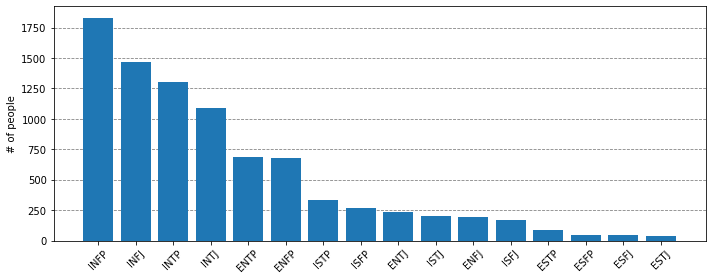
\includegraphics[width=0.9\linewidth]{../report/fig/distribution.png}
\caption{各类性格分布}
\label{fig:distribution}
\end{figure}

由于sklearn自带的数据集划分方式均无法解决这种类别不均的采样问题,因此我自己写了一个训练集生成器,用于划分出均匀的训练集和测试集。

\lstinputlisting[firstline=242,lastline=268]{../SVM.py}

这里相当于在每个类别内部进行随机抽样划分,但确保每个类别都能在训练集和测试集中出现,这样可以更好衡量模型的真实泛化性能,而不会出现某个类别缺失而导致预测正确率偏高的情况。

\section{实验结果}
本次实验的完整代码可见附件中的\verb'SVM.ipynb'或由Jupyter Notebook生成的\verb'SVM.py'文件。

\subsection{超参数选择}
实验所采用的超参数如表\ref{tab:hyperparam}所示。
之所以要设置词典最小词频,是为了减少特征维度,进而缩短训练时间。
\begin{table}[H]
\caption{超参数设置}
\label{tab:hyperparam}
\centering
\begin{tabular}{|c|c|}\hline
词典最小词频 & 20 \\\hline
Word2Vec词向量维度 & 512 \\\hline
L2正则化参数$C$ & 1\\\hline
SVM核 & Linear\\\hline
\end{tabular}
\end{table}

生成的特征矩阵维度为$8676\times 13489$,前者为用户数目,后者为词典大小。

\subsection{综合比较}
最终各类别的F1及精确度指标如图\ref{fig:f1}所示,可以看到我的SVM最终达到了64.94\%的准确率,比上次随机森林的性能翻了整整一倍。
\begin{figure}[H]
\centering
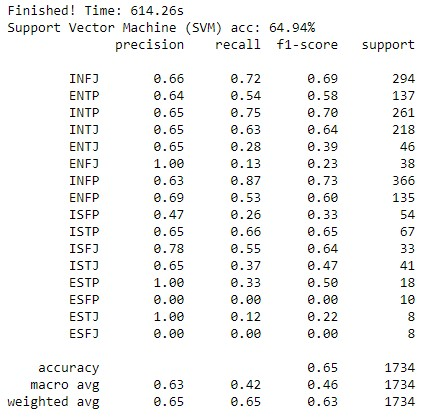
\includegraphics[width=0.8\linewidth]{fig/tfidf-svm-f1-small.jpg}
\caption{实验结果}
\label{fig:f1}
\end{figure}

同时由于采用了均匀类别划分方式,除了极少数类别如ESFP和ESFJ,其他类别都能够部分正确地预测出来。
当然,随着样本的增加,预测准确率也更高,这一点依然从表中会呈现出来,这与图\ref{fig:distribution}的分布类似,因此这也提醒我们要着重关注那些少样本的类别。

对于不同词嵌入方法及不同机器学习模型的性能比较可见图\ref{fig:comparison}。
\begin{figure}[H]
\centering
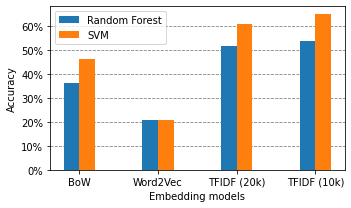
\includegraphics[width=0.6\linewidth]{fig/comparison.png}
\caption{随机森林与SVM在不同词嵌入方法下的准确率比较}
\label{fig:comparison}
\end{figure}

从图中可以看出采用词袋模型或者TF-IDF模型,预测准确率都比较高;而采用Word2Vec进行嵌入,机器学习模型几乎学不到东西。
这很大一部分原因是词袋模型和TF-IDF模型的特征维度非常巨大,达到了万维,尽管大量是0元素,但是对于机器学习模型来说可能也是很重要的学习的一部分;而在训练Word2Vec模型时,我只采用了512维的特征空间,因此相比起来能够获取的用户词语信息就变少了,且还是被压缩降维后的信息,因此效果不好也可以理解。

对于词袋模型和TF-IDF模型的比较,TF-IDF还是比词袋模型胜出了至少10个百分点,这也是因为其考虑了不同词语的重要性,以让机器更好地捕获特征。
但比较出人意料的是,随着TF-IDF模型特征维度的减少(通过词典最小词频控制),其预测准确率不降反升,这或许是长尾效应,大部分尾部的词语并没有带来太多的信息量,甚至可能会干扰决策,因此直接将这些单词去除,反而会有利于机器学习模型去学习。

总的来说,虽然SVM比随机森林的预测准确率要稍高,但是其计算的时间复杂度实在太高了,对于本问题这种维度破万的特征,需要耗费大量的时间进行训练。
在实验中会发现,随机森林的训练时间基本在0.1秒,而SVM至少需要10分钟,而且还是都开了并行的情况下的运算。
也就是说,随机森林的速度比SVM快了6000倍,这其实更适合对于时间要求较高的应用。

\section{总结与思考}
本次作业的两个实验都需要灵活使用上学期自然语言处理课程的知识来进行处理,后面的机器学习的模型实现、训练与调参反倒不是最为重要的,因为这些都有现成的理论和工具,只要慢慢调整复现即可。

而经过这一次实验就会发现,采用什么词向量模型对最终结果的影响是巨大的,这其实属于特征工程的部分,某种意义上验证了那句老话,“有多少人工就有多少智能”。
只有前面的数据集清洗得好,同时采用合适的特征构造选择方式,后面的机器学习模型才有办法从中学到东西并做出合理预测。

\begin{thebibliography}{99}
\bibitem{bib:tfidf} Wikipedia, TF-IDF, \url{https://en.wikipedia.org/wiki/Tf%E2%80%93idf}
\bibitem{bib:word2vec} Tomas Mikolov, Ilya Sutskever, Kai Chen, Greg Corrado, and Jeffrey Dean, \emph{Distributed Representations of Words and Phrases and their Compositionality}, NeurIPS, 2013
\end{thebibliography}
% https://stackabuse.com/python-for-nlp-creating-tf-idf-model-from-scratch/
% https://stackoverflow.com/questions/31681373/making-svm-run-faster-in-python

\end{document}

% 作业内容:
% 1. 使用集成学习方法完成人格分类(6月10日)
% * 对数据进行预处理
% * 使用集成学习模型(AdaBoost或Random Forest)进行人格分类
% * 提交报告及代码
% 2. 使用SVM进行人格分类(6月30日)
% * 数据预处理
% * 使用SVM进行人格分类
% * 提交报告及代码
% ** 加分项:使用英文撰写报告,设计合理实验(对比不同模型表现/不同超参数对性能的影响),自己撰写模型代码,尽可能少调用工具

% 评价指标:
% * 单独对每种类别进行评价/整体评价
% * F1 \& Accuracy

% 评分:
% * 集成学习方法:20分
% * SVM方法:20分